\chapter{Modelagem do Sistema}

Neste capítulo, apresentamos a modelagem do sistema, detalhando sua infraestrutura e o fluxo de dados entre os diferentes componentes. A modelagem inclui a interação do usuário com a interface de gerenciamento, a comunicação com o servidor central e a coleta de dados realizada pelos agentes instalados nos dispositivos monitorados. A Figura \ref{fig:Infrasis1} ilustra a infraestrutura completa, destacando o fluxo de informações desde o usuário até os bancos de dados centralizados, garantindo a rastreabilidade e integridade das informações.


\begin{figure}[h]
    \centering
    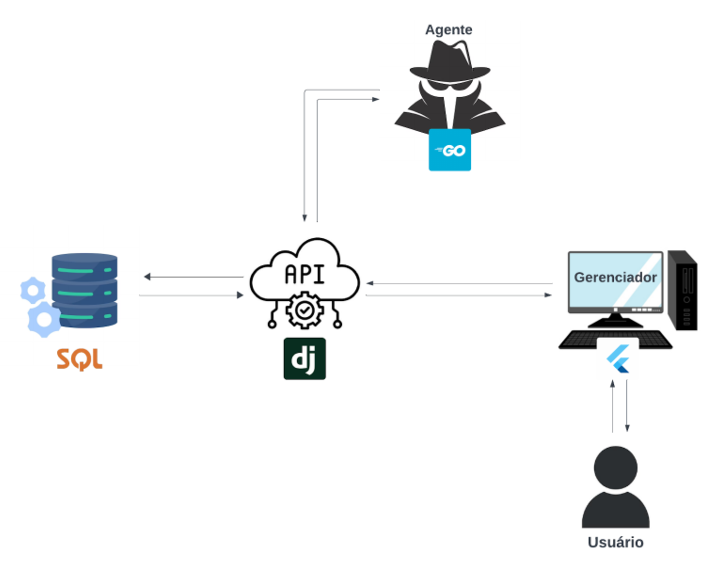
\includegraphics[width=1\linewidth]{figuras/modelagemArc.png}
    \caption{Arquitetura da infraestrutura do sistema}
    \label{fig:Infrasis1}
\end{figure}
Além disso, discutiremos a estruturação do trabalho, incluindo o backlog, o diagrama de classes. A seguir, detalhamos o processo de desenvolvimento e as tecnologias básicas utilizadas para construir nosso sistema.

\section{Planejamento do Desenvolvimento}

Para a construção do sistema, adotamos uma abordagem modular, dividindo o desenvolvimento em três principais componentes: Interface de Gerenciamento Desktop, Servidor Central e Agentes Distribuídos. Cada componente foi cuidadosamente planejado para atender aos requisitos de escalabilidade, eficiência e segurança.  

A interface de gerenciamento foi projetada para oferecer uma experiência de usuário intuitiva, facilitando a visualização e o controle dos ativos. O servidor central foi planejado para gerenciar o armazenamento e o processamento de dados de maneira segura e confiável. Por fim, os agentes distribuídos foram desenvolvidos para capturar informações diretamente dos dispositivos monitorados e comunicar essas informações ao servidor.  

Optamos por definir as tecnologias e frameworks ao longo do processo de implementação, permitindo maior flexibilidade para adaptar as escolhas às necessidades específicas de cada componente e garantir um desempenho otimizado do sistema.


\section{Requisitos de Referência}
Elaboramos uma lista de requisitos para servir como referência na construção do projeto, definindo as principais funcionalidades e características necessárias para atender às demandas identificadas.
\subsection{Requisitos de Negócio}
\begin{itemize}
    \item RN1: O sistema deve otimizar a gestão de ativos de TI, reduzindo o tempo necessário para localizar, atualizar ou consultar informações sobre os equipamentos.
    \item RN2: O sistema deve centralizar todas as informações sobre ativos de TI, incluindo dados de localização, usuários e licenças de software, para facilitar a tomada de decisão.
    \item RN3: O sistema deve permitir um monitoramento em tempo real dos ativos de TI, possibilitando a identificação rápida de problemas operacionais ou desvios no uso de equipamentos.
    \item RN4: O sistema deve registrar um histórico completo de mudanças nos ativos, incluindo troca de localização, alterações de configuração e instalação de softwares, para garantir rastreabilidade e conformidade com auditorias.
    \item RN5: O sistema deve aumentar a eficiência operacional da equipe de TI, reduzindo a necessidade de processos manuais e simplificando a administração dos recursos tecnológicos.
    \item RN6: O sistema deve garantir que todos os ativos de TI estejam devidamente licenciados e que as relações de licenciamento sejam atualizadas automaticamente para evitar problemas legais e financeiros.
    \item RN7: O sistema deve ser escalável e adaptável para atender à expansão da organização, seja com o aumento de equipamentos monitorados ou com a adição de novos locais.
    \item RN8: O sistema deve oferecer segurança robusta para proteger as informações sensíveis dos ativos de TI e evitar acessos não autorizados.
    \item RN9: O sistema deve permitir a análise de dados gerados pelos agentes e pelo histórico de ativos para identificar padrões, prever necessidades futuras e gerar relatórios estratégicos.
    \item RN10: O sistema deve reduzir custos operacionais relacionados à perda de equipamentos, redundância de licenças ou uso ineficiente de recursos tecnológicos. 
    \item RN11: O sistema deve possibilitar o gerenciamento de ativos em ambientes distribuídos, como campi ou filiais, garantindo uma visão centralizada e integrada.
\end{itemize}

\subsection{Requisitos de Usuário}
\begin{itemize}
\item RU1: O usuário deve ser capaz de acessar uma interface gráfica intuitiva para visualizar, cadastrar, editar e desativar ativos de TI.  
    \item RU2: O usuário deve conseguir localizar rapidamente ativos de TI por filtros como tipo, localidade, ou usuário associado.  
    \item RU3: O usuário deve ter acesso a uma visualização gráfica interativa da planta baixa, podendo identificar ativos em tempo real e obter informações detalhadas ao clicar em um ativo.  
    \item RU4: O usuário deve poder registrar manualmente novos ativos de TI no sistema, incluindo informações como patrimônio, localização, e responsável.  
    \item RU5: O usuário deve ser capaz de monitorar o status de funcionamento dos ativos, como se estão ligados, desligados ou inativos.  
    \item RU6: O usuário deve poder rastrear o histórico de mudanças de localização e configuração de cada ativo.  
    \item RU7: O usuário deve ter a opção de vincular ativos entre si, como associar monitores, periféricos ou softwares a uma máquina específica.  
    \item RU8: O usuário deve conseguir aprovar novos agentes conectados ao sistema, garantindo que apenas dispositivos autorizados sejam monitorados.  
    \item RU9: O usuário deve poder visualizar relatórios e dashboards que apresentem informações consolidadas sobre os ativos de TI, como número de ativos por localidade, status operacional e licenças utilizadas.  
    \item RU10: O usuário deve ser notificado em caso de falhas no sistema ou quando um ativo estiver inativo por um período prolongado.  
    \item RU11: O usuário deve poder editar informações associadas a ativos, como alteração de local, troca de usuário responsável ou atualização de especificações técnicas.  
    \item RU12: O usuário deve ter acesso a ferramentas de busca e filtros avançados para localizar rapidamente ativos específicos.  
    \item RU13: O usuário deve conseguir realizar alterações no sistema sem a necessidade de conhecimentos avançados de TI, graças a um design centrado na usabilidade.  
    \item RU14: O usuário deve poder configurar níveis de acesso para diferentes perfis de utilização, garantindo que dados sensíveis sejam protegidos de acessos não autorizados.  
    \item RU15: O usuário deve ter suporte para registrar o motivo de trocas de localidade, facilitando o rastreamento de justificativas.  
    \item RU16: O usuário deve poder acessar o sistema de diferentes locais e dispositivos, desde que tenha as permissões adequadas.  
    \item RU17: O usuário deve poder utilizar o sistema para verificar a conformidade de licenças de software instaladas nos dispositivos monitorados.  
\end{itemize}


\subsection{Requisitos Funcionais}

Os requisitos funcionais de um sistema descrevem as funcionalidades e comportamentos específicos que ele deve executar para atender às necessidades do usuário. Eles definem o que o sistema deve fazer, como processar entradas e gerar saídas, e como deve interagir com usuários e outros sistemas.

\subsubsection{CRUD de Ativos de TI}
\begin{itemize}
    \item RF1: O sistema deve exibir uma listagem completa de todos os ativos de TI cadastrados.
    \item RF2: O sistema deve permitir a inserção manual de novos ativos de TI.
    \item RF3: O sistema deve permitir a edição das informações de ativos de TI previamente cadastrados.
    \item RF4: O sistema deve permitir a visualização detalhada das informações de um ativo de TI específico.
    \item RF5: O sistema deve permitir a desativação de ativos de TI, mantendo o histórico do ativo no sistema.
\end{itemize}

\subsubsection{Visualização Gráfica Espacial dos Ativos de TI}
\begin{itemize}
    \item RF7: O sistema deve listar as salas e setores dentro de um campus, com opções de filtro por bloco e sala/setor.
    \item RF8: O sistema deve exibir interativamente a planta baixa de uma sala, com botões representando as CPUs; ao clicar em um botão, deve abrir um modal contendo informações em tempo real sobre o PC e o usuário logado.
\end{itemize}

\subsubsection{Agente de Ativo de TI}
\begin{itemize}
    \item RF9: O sistema deve incluir um programa instalado em cada CPU, que se integra automaticamente ao sistema de gerenciamento ao se conectar, sem interface gráfica.
    \item RF10: O sistema deve exigir que cada agente utilize uma chave API para se autenticar.
    \item RF11: O sistema deve permitir que novos agentes sejam validados e aprovados pelo gerenciador antes de serem integrados.
    \item RF12: O sistema deve permitir que o agente envie automaticamente dados como patrimônio, IP, usuário logado e informações técnicas do PC.
    \item RF13: O sistema deve monitorar continuamente e reportar se o PC está ligado ou desligado.
    \item RF14: O sistema deve criar automaticamente novos ativos para cada software licenciado instalado nos PCs.
\end{itemize}

\subsubsection{Gerência de Ativo de TI}
\begin{itemize}
    \item RF15: O sistema deve permitir a troca de local de um ativo de TI, com um campo para explicar o motivo da troca.
    \item RF16: O sistema deve manter um histórico das trocas de local para cada ativo de TI.
    \item RF17: O sistema deve permitir vincular um ativo de TI a outro, como vincular softwares a um computador ou monitores a um computador.
\end{itemize}


\subsection{Requisitos Não Funcionais}

Os requisitos não funcionais descrevem como o sistema deve funcionar, focando em qualidades e restrições que impactam o desempenho e a usabilidade, mas não diretamente nas funcionalidades.

\begin{itemize}
    \item RNF1: O sistema deve processar solicitações e integrar agentes com alta performance.
    \item RNF2: O sistema deve ser escalável para suportar crescimento de ativos e usuários.
    \item RNF3: O sistema deve garantir segurança em dados, comunicações e acessos.
    \item RNF4: O sistema deve ser intuitivo e acessível para todos os usuários.
    \item RNF5: O sistema deve ser altamente confiável com disponibilidade de 99,9\%.
    \item RNF6: O sistema deve ser modular e fácil de manter e atualizar.
    \item RNF7: O agente deve ser compatível com o sistema operacional Windows.
    \item RNF8: O sistema deve ser compatível com os sistemas operacionais Windows e Linux.
\end{itemize}



\section{Tecnologias Básicas}

Nesse momento, escolhemos quais seriam as tecnologias-base para, em um outro momento, iniciarmos a implementação.

\subsection{Interface de Gerenciamento Desktop}

\begin{itemize}
    \item \textbf{Flutter:} Framework desenvolvido pelo Google para a construção de interfaces gráficas modernas e responsivas. Escolhido por sua capacidade de desenvolver aplicações desktop multiplataforma com alto desempenho.
    \item \textbf{Dart:} Linguagem de programação utilizada pelo Flutter, reconhecida por sua facilidade de uso e performance otimizada para interfaces gráficas.
\end{itemize}

\subsection{Back-end}

\begin{itemize}
    \item \textbf{Python:} Linguagem de programação escolhida para o desenvolvimento do back-end devido à sua simplicidade e robustez.
    \item \textbf{Django:} Framework web de alto nível para Python, que facilita o desenvolvimento rápido e seguro de aplicações web.
\end{itemize}

\subsection{Agente Desktop}

\begin{itemize}
    \item \textbf{Golang (Go):} Linguagem de programação escolhida para o desenvolvimento do agente desktop devido à sua eficiência, baixo consumo de recursos e suporte nativo para concorrência. Ideal para a coleta e envio contínuo de dados ao servidor.
\end{itemize}

\subsection{Banco de Dados em Nuvem}

Optamos pelo uso de bancos de dados em nuvem devido à sua escalabilidade, segurança e facilidade de gerenciamento. A escolha específica do banco de dados será determinada com base nas necessidades do projeto e nos custos associados.

\subsection{Infraestrutura e Fluxo de Dados}

A Figura \ref{fig:Infrasis1} apresenta a infraestrutura do sistema, destacando o fluxo de dados desde a interação do usuário na interface desktop até o armazenamento e processamento no banco de dados em nuvem. A modelagem considera a segurança dos dados, a escalabilidade do sistema e a eficiência na comunicação entre os diferentes componentes.


\section{Estruturação do Software}



\subsection{Diagrama de Classes}

O diagrama de classes é uma representação visual das classes do sistema e suas interações. Ele ajuda a entender a estrutura do código, as relações entre as classes e a organizar o desenvolvimento do software de maneira mais eficiente.

\begin{figure}[H]
    \centering
    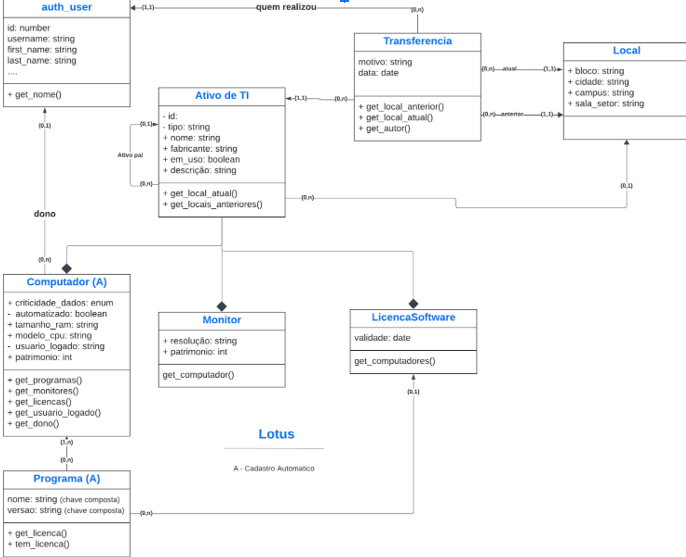
\includegraphics[width=0.8\linewidth]{figuras/diagramaclasses.png}
    \caption{Diagrama de classes}
    \label{fig:classes}
\end{figure}

Conforme ilustrado na Figura \ref{fig:classes} acima, optamos por uma abordagem simplificada de classes para mitigar a complexidade no sistema, especialmente devido ao tempo limitado previsto no cronograma de implementação.

\subsection{Diagrama Entidade-Relacionamento (ER)}
O Diagrama Entidade-Relacionamento (ER) é uma representação visual que mostra como os dados estão relacionados em um sistema. Ele modela entidades (objetos ou conceitos importantes para o sistema) e seus relacionamentos. Cada entidade tem atributos que representam suas propriedades, e as relações entre as entidades indicam como elas interagem entre si. O objetivo do diagrama ER é ajudar no planejamento e compreensão da estrutura do banco de dados, facilitando o design e a implementação.

\begin{figure}[H]
    \centering
    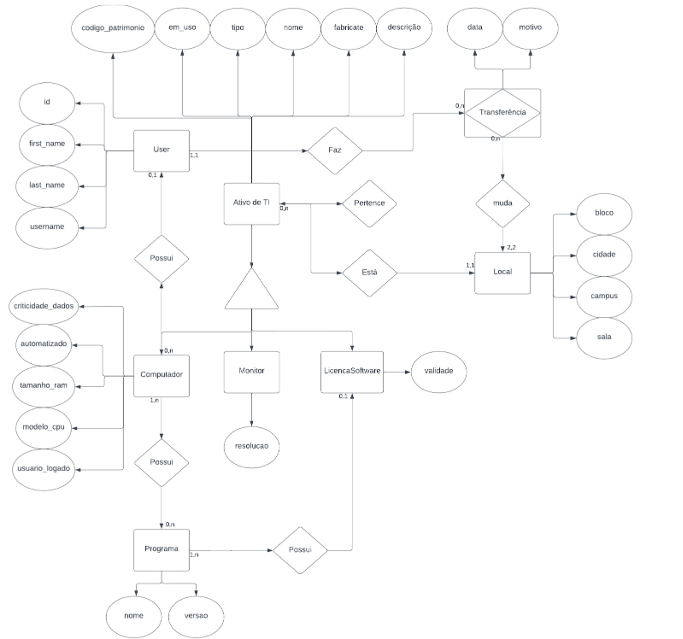
\includegraphics[width=0.8\linewidth]{figuras/DIAGRAMAer.png}
    \caption{Diagrama ER}
    \label{fig:classes}
\end{figure}


\section{Wireframe Front-End Desktop}
Este protótipo exibe todos os ativos cadastrados no sistema, organizados em uma lista com as principais informações de cada item.

\begin{figure}[H]
    \centering
    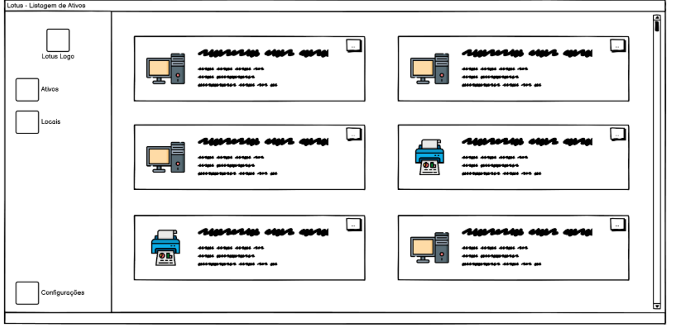
\includegraphics[width=1\linewidth]{figuras/lsitagemativos.png}
    \caption{Listagem de ativos}
    \label{fig:mockup1}
\end{figure}

Ao selecionar um ativo na listagem, esta interface apresenta informações detalhadas sobre o ativo, incluindo descrição, localização e relações com outros ativos.


\begin{figure}[H]
    \centering
    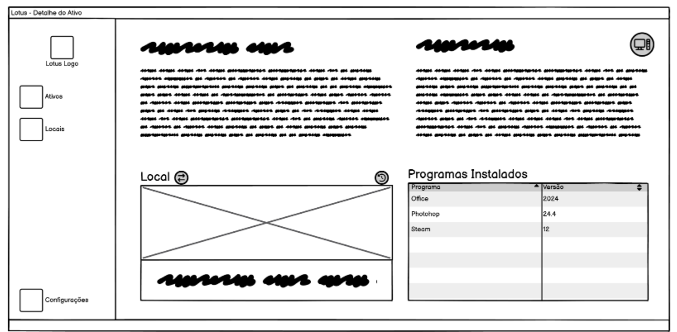
\includegraphics[width=1\linewidth]{figuras/detalhesativo.png}
    \caption{Detalhes do Ativo}
    \label{fig:mockup2}
\end{figure}

Neste modal, o usuário poderá alterar a localização de um ativo específico. A funcionalidade permite a rápida atualização da posição de um ativo no sistema.


\begin{figure}[H]
    \centering
    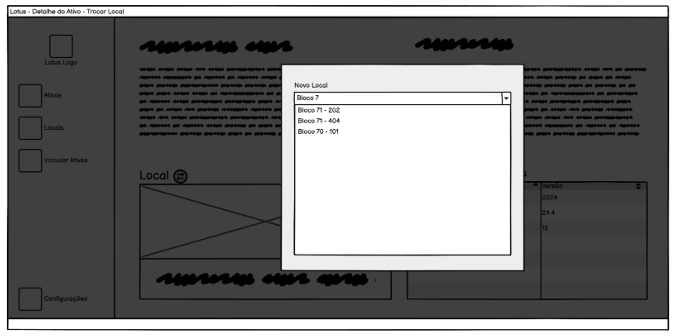
\includegraphics[width=1\linewidth]{figuras/trocarativo.png}
    \caption{Trocar Local do Ativo}
    \label{fig:mockup3}
\end{figure}

Este modal possibilita a associação entre diferentes ativos, formando grupos lógicos. A vinculação facilita o gerenciamento de ativos relacionados.


\begin{figure}[H]
    \centering
    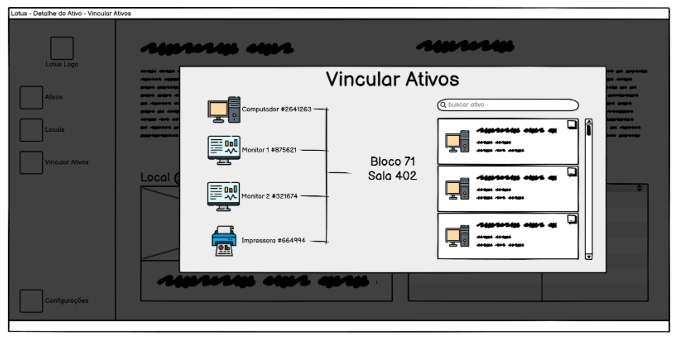
\includegraphics[width=1\linewidth]{figuras/vincularativo.png}
    \caption{Vincular Ativos}
    \label{fig:mockup3}
\end{figure}

Neste protótipo, o usuário pode visualizar todos os locais registrados no sistema, organizados de forma clara para facilitar a navegação e busca.


\begin{figure}[H]
    \centering
    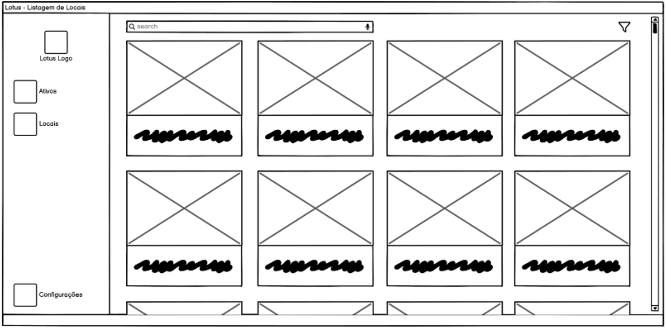
\includegraphics[width=1\linewidth]{figuras/listarlocais.png}
    \caption{Listagem de Locais}
    \label{fig:mockup3}
\end{figure}

Este protótipo oferece uma visão detalhada de um local específico. Inclui uma visualização espacial dos ativos alocados, exibindo sua posição em um mapa.

\begin{figure}[H]
    \centering
    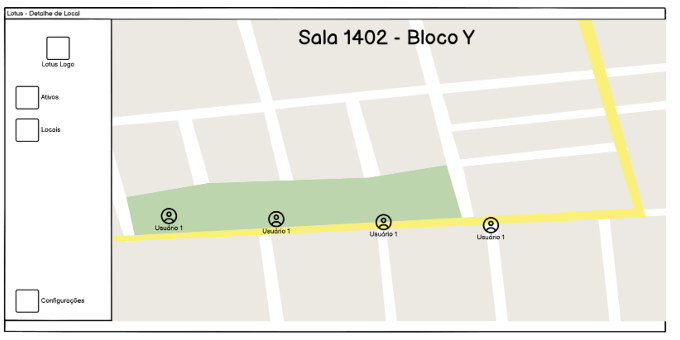
\includegraphics[width=1\linewidth]{figuras/detalheslocal.png}
    \caption{Detalhe de Local}
    \label{fig:mockup3}
\end{figure}


Optamos por criar alguns wireframes básicos para obtermos uma ideia inicial do design da nossa aplicação desktop. Esses wireframes são essenciais para visualizarmos como os diferentes elementos da interface serão organizados e interagirão entre si, antes de iniciarmos a implementação detalhada. Eles nos ajudarão a validar conceitos de usabilidade, identificar possíveis melhorias e alinhar expectativas sobre o visual e a funcionalidade da aplicação.




\section{Conclusão da Modelagem do Sistema}

Nesta etapa, detalhamos a modelagem do sistema, destacando as tecnologias básicas, a infraestrutura planejada e a estruturação do trabalho, incluindo o diagrama de classes.
